\chapter{Desarrollo de APIs}

En este capítulo se hablará sobre las diferentes librerías (APIs) que se han realizado en este proyecto, explicando detalladamente la estructura de cada una de ellas.

Por último, se hará especial énfasis en el plugin de Net2Plan desarrollado, en el cual se han integrado las difrentes APIs mencionadas anteriormente.


\section{J-OSM Client}
\label{sec:osmclient}

J-OSMClient es una librería programada en Java cuya funcionalidad es la de proporcionar un cliente REST para interactuar con OSM (ver sección \ref{sec:osm}).

\begin{figure}[!ht]
	\centering
	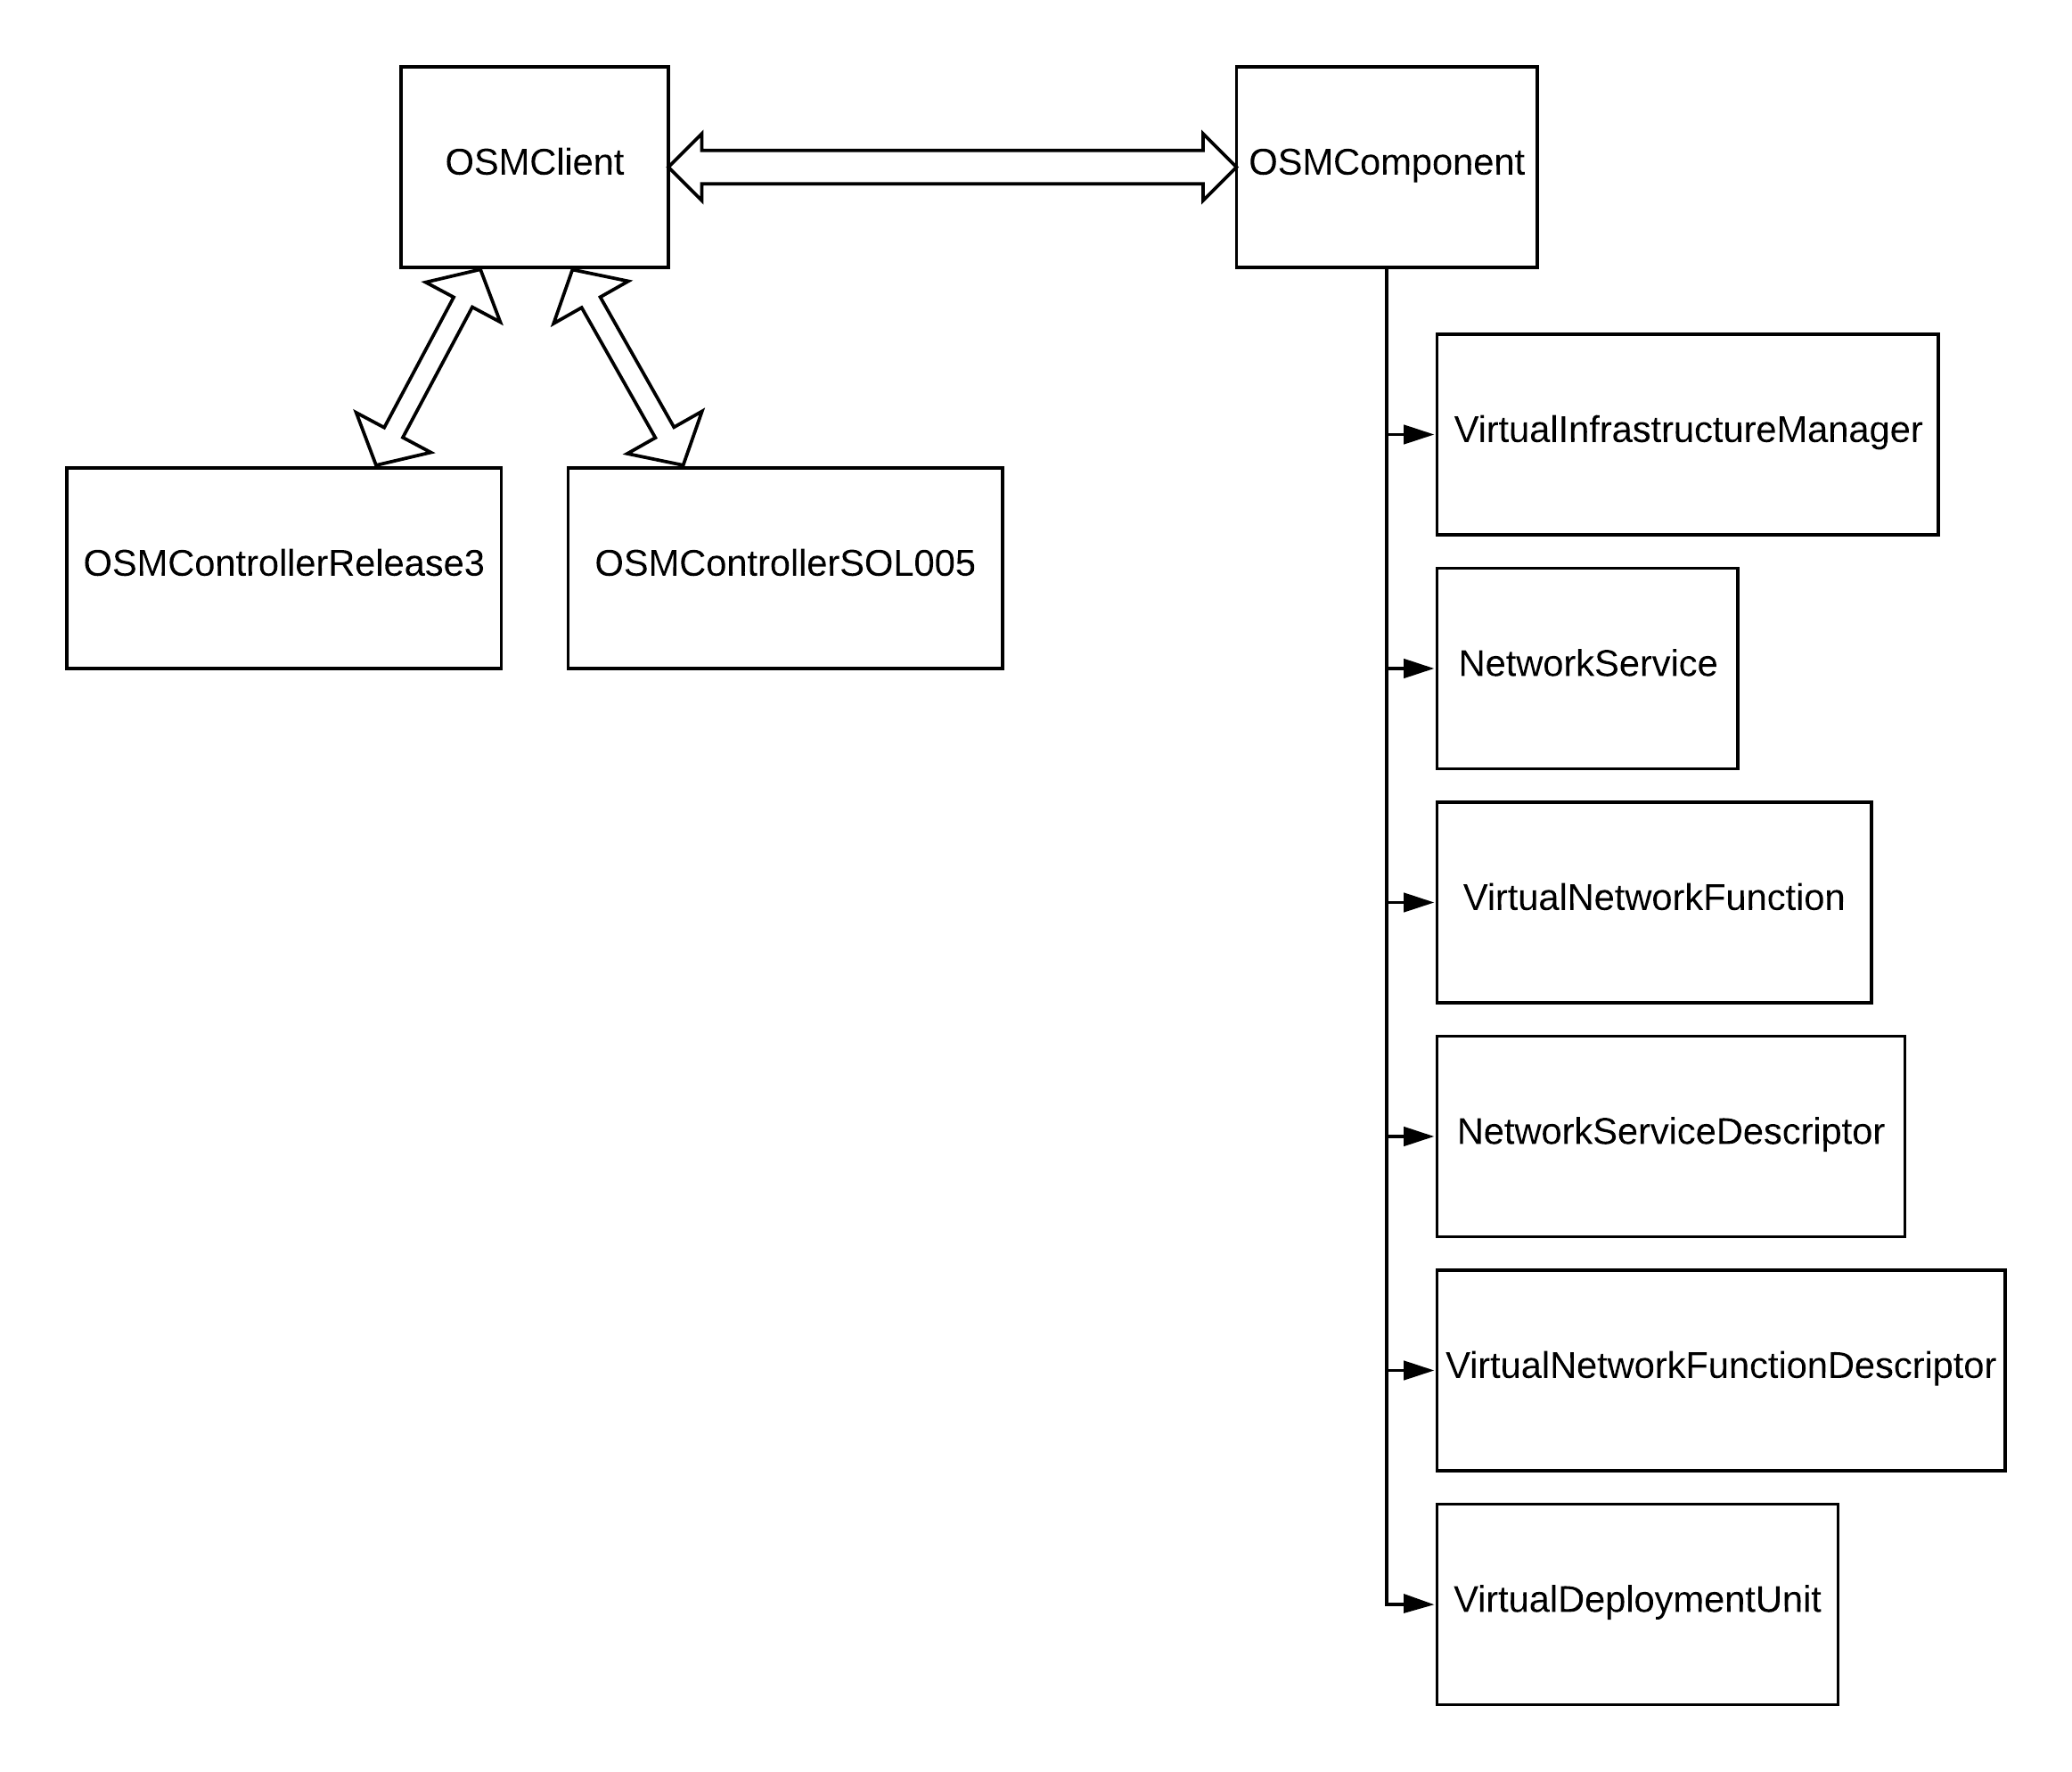
\includegraphics[width=0.8\linewidth]{imagenes/OSMClient}
	\caption{Estructura de clases de J-OSMClient}
	\label{fig:osmclient}
\end{figure}

En la figura \ref{fig:osmclient} se puede ver un esquema detallado de la jerarquía de clases y como dichas clases interaccionan entre sí.


\section{ONOS Client}
\label{sec:onosclient}

\begin{figure}[!ht]
	\centering
	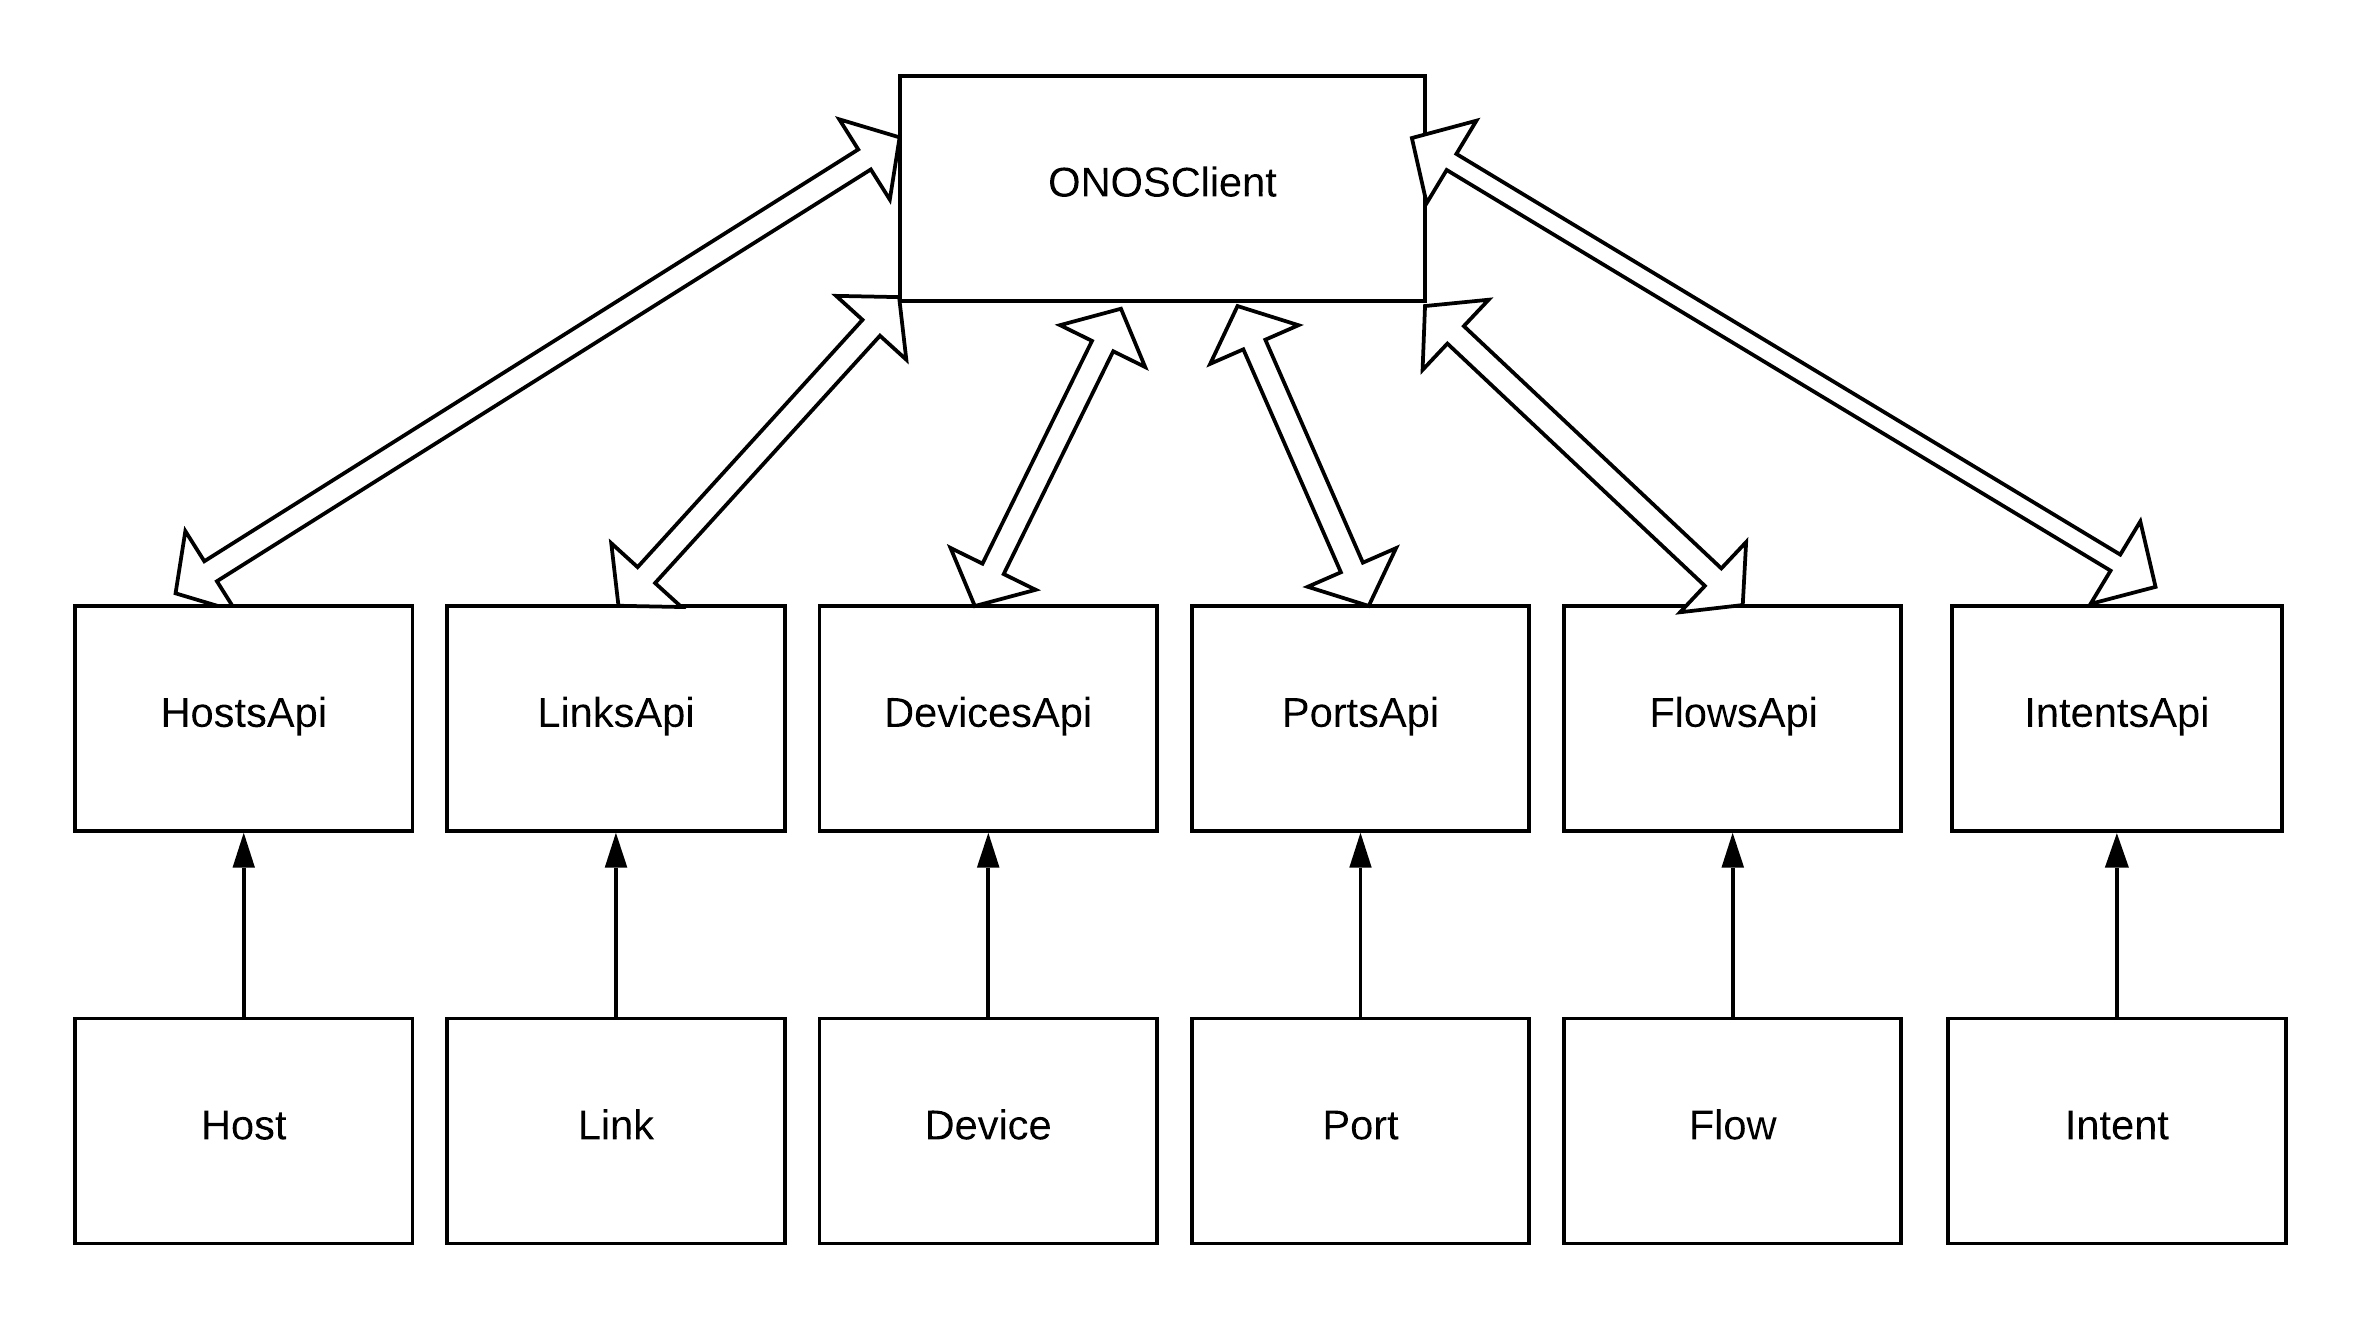
\includegraphics[width=0.8\linewidth]{imagenes/ONOSClient}
	\caption{Estructura de clases de ONOSClient}
	\label{fig:onosclient}
\end{figure}


\section{OpenStack Client}
\label{sec:openstackclient}

\begin{figure}[!ht]
	\centering
	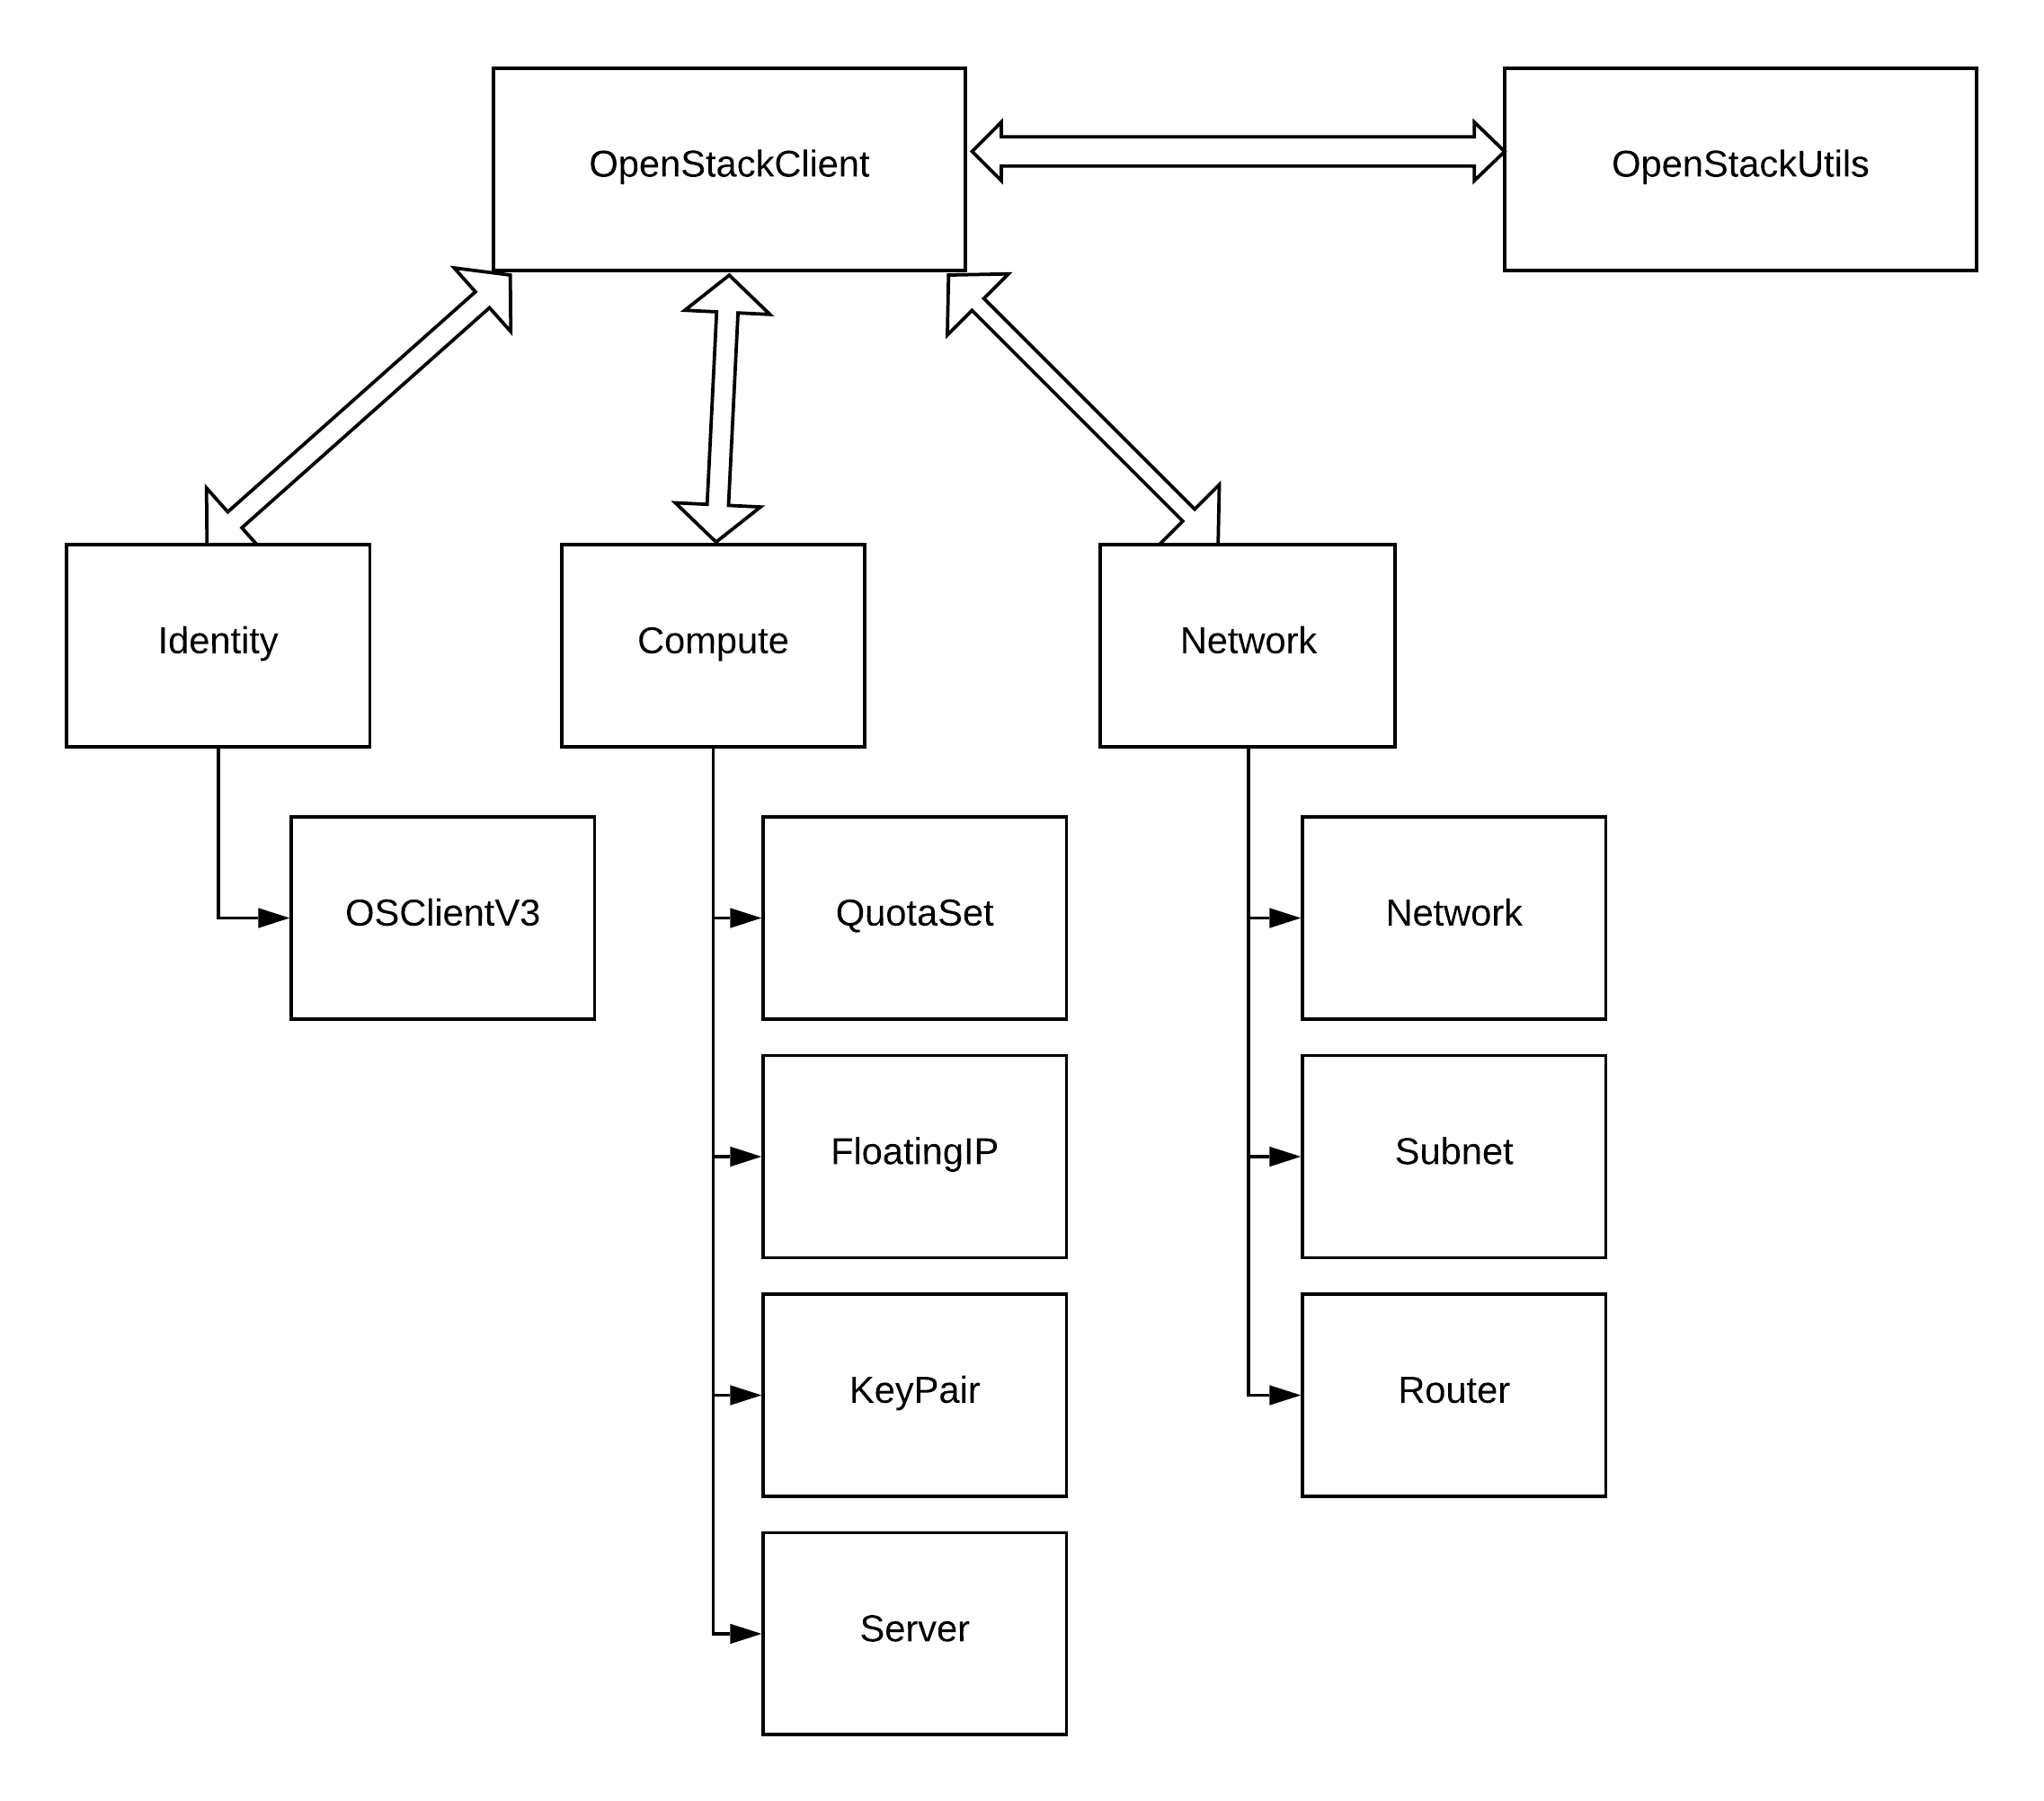
\includegraphics[width=0.8\linewidth]{imagenes/OpenStackClient}
	\caption{Estructura de clases de OpenStackClient}
	\label{fig:openstackclient}
\end{figure}

\section{Net2Plan: NFV Management Plugin}
\label{sec:nfvplugin}

Para llevar a cabo este proyecto, era necesario integrar las APIs mencionadas anteriormente con una herramienta que tenga funcionalidad de planificación de redes. Por ello, se ha desarrollado una extensión de Net2Plan basada en el plugin Network Design, cuya página de inicio se puede observar en la figura \ref{fig:nfvpluginmain}.

\begin{figure}[!ht]
	\centering
	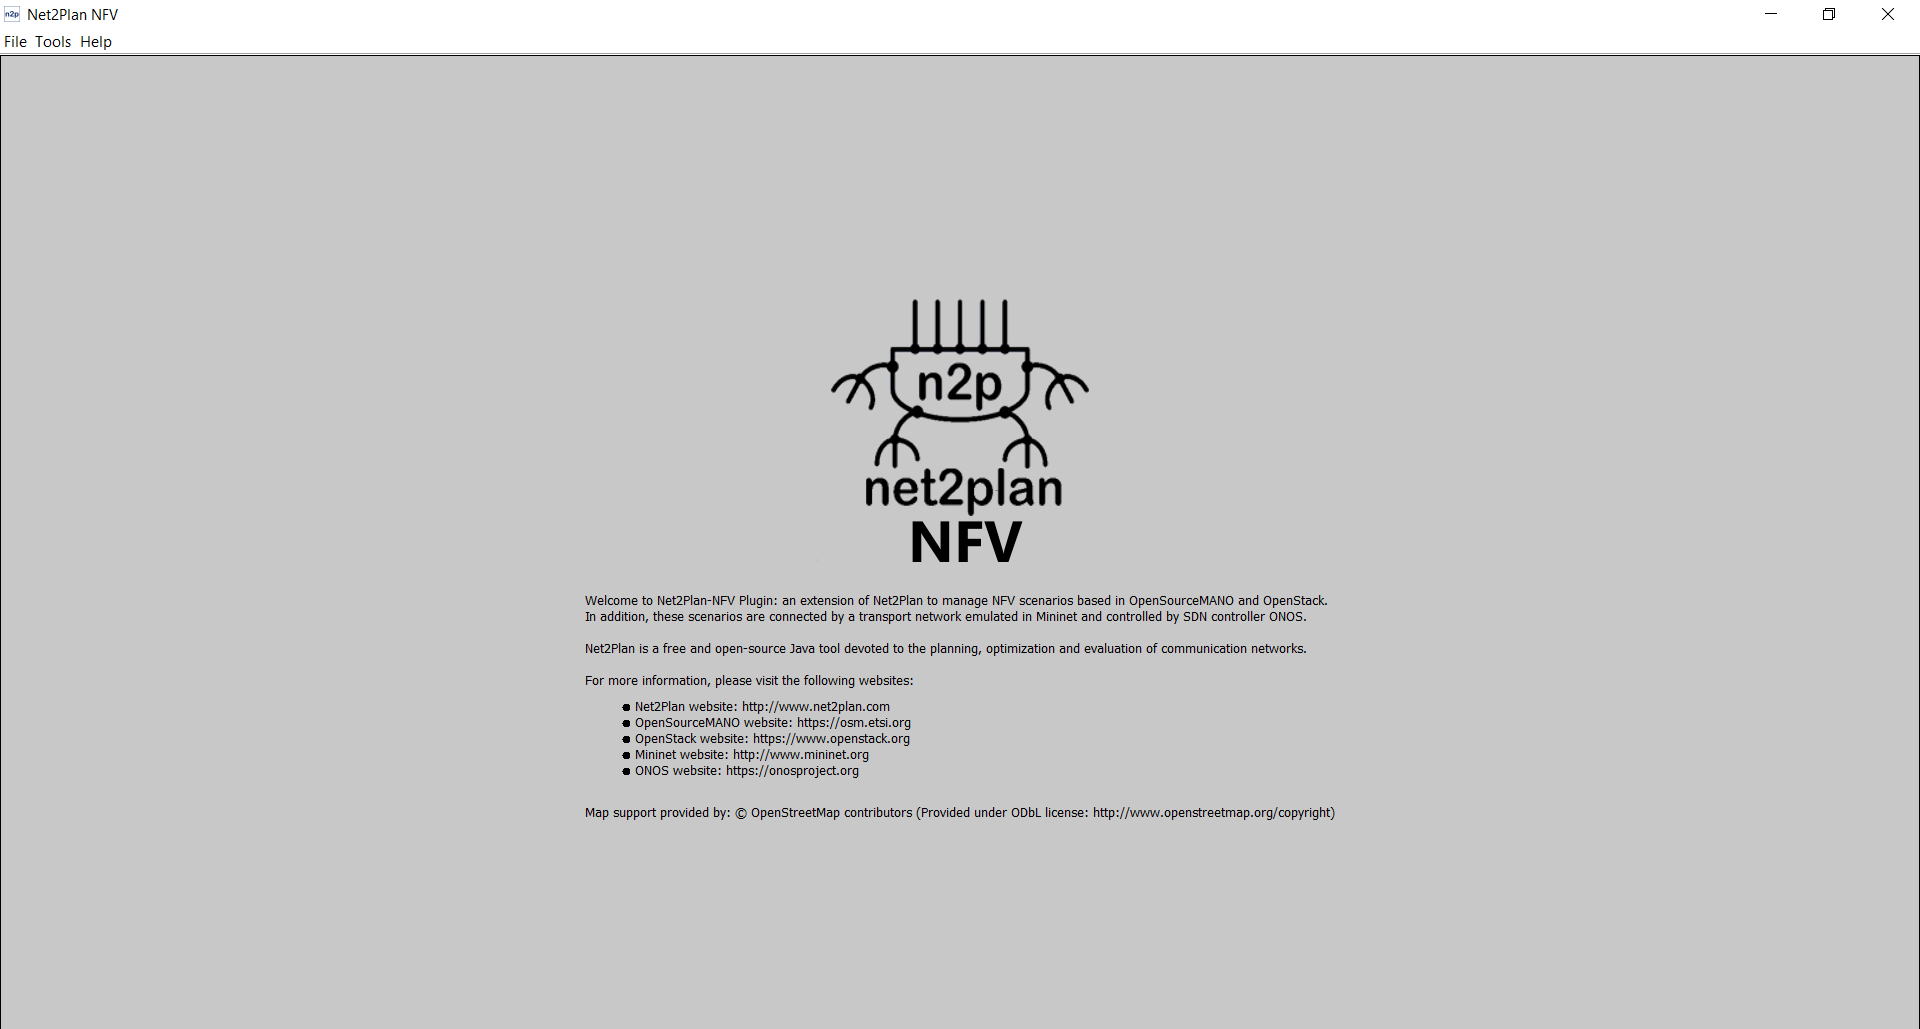
\includegraphics[width=0.8\linewidth]{imagenes/nfvpluginmain}
	\caption{Página de inicio de la extensión Net2Plan-NFV}
	\label{fig:nfvpluginmain}
\end{figure}


\begin{figure}[!ht]
	\centering
	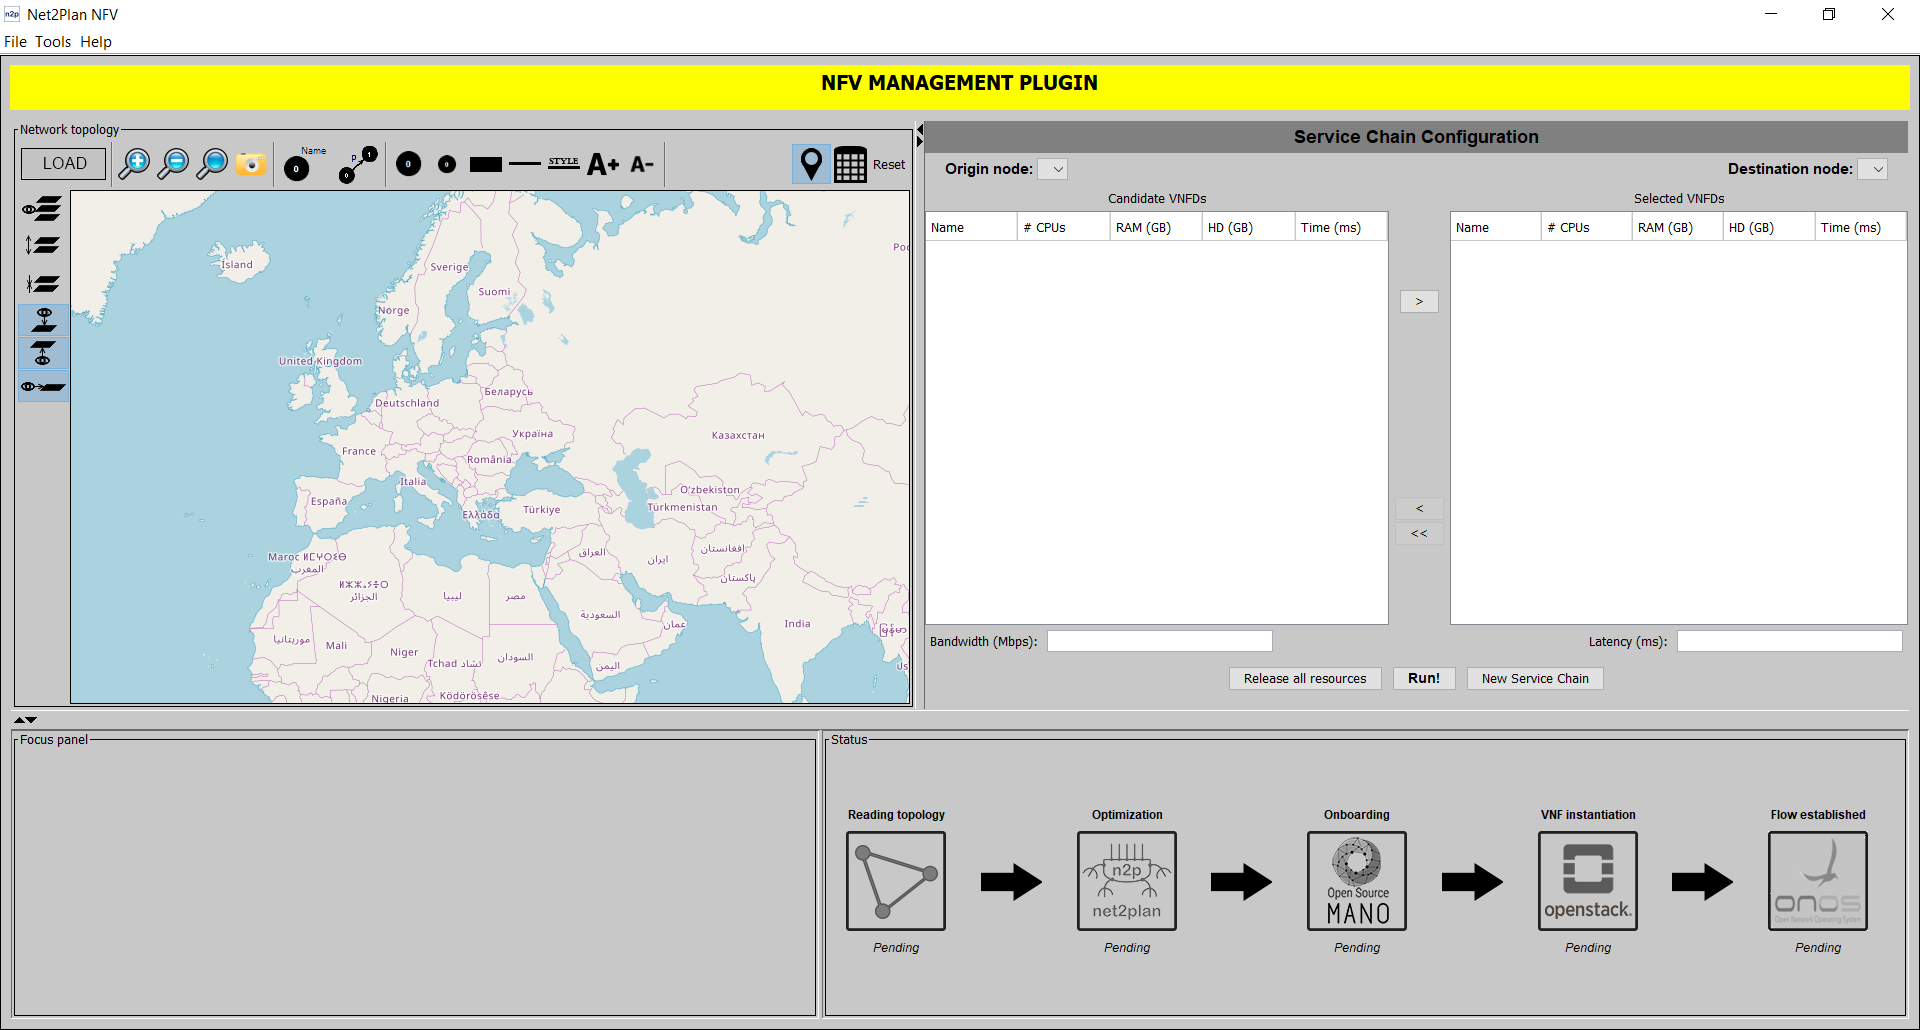
\includegraphics[width=0.8\linewidth]{imagenes/nfvplugin_dashboard}
	\caption{Interfaz gráfica del Plugin NFV-Management}
	\label{fig:nfvplugindash}
\end{figure}

Así mismo, en la figura \ref{fig:nfvplugindash} se puede observar la interfaz gráfica del Plugin NFV-Management, la cual está dividida en diferentes secciones:

\begin{itemize}
	\item Arriba a la izquierda se encuentra el \textit{TopologyPanel}, que se encarga de dibujar la topología deseada. Esta funcionalidad es heredada del \textit{Plugin Network Design} de Net2Plan.
	
	\item Arriba a la derecha se encuentra el \textit{OSMPane}l, que se encarga de obtener información sobre los distintos NSD que se encuentran disponibles en OSM y mostrarla al usuario de una manera amigable, informándole de que recursos (HD, RAM, CPU) son necesarios para su instanciación en un VIM.
	
	\item Abajo a la izquierda se encuentra el \textit{FocusPanel}, que se encarga de mostrar información detallada de un elemento en concreto cuando se selecciona. Dicha funcionalidad es heredada del \textit{Plugin Network Design} de Net2Plan.
	
	\item Abajo a la derecha se encuentra el \textit{ServiceChainPanel}.
\end{itemize}




\cleardoublepage